\paragraph{Indice di Gulpease}\mbox{}\\[0,3cm]
\begin{table}[H]
	\centering
	\begin{tabular}{cccc}
	\rowcolor{greySWEight}
	\textcolor{white}{\textbf{Documento}} & 
	\textcolor{white}{\textbf{Abbreviazione}} &
	\textcolor{white}{\textbf{Valore Indice}}&
	\textcolor{white}{\textbf{Riscontro}}\\
	
	\textbf{Analisi dei Requisiti} &
	ADR & 
	54 &
	\textcolor{ForestGreen}{Ottimale}
	\\
	\textbf{Glossario} &
	GLO &
	60 &
	\textcolor{ForestGreen}{Ottimale}
	\\	
	\textbf{Piano di Progetto} &
	PDQ &
	70 &
	\textcolor{ForestGreen}{Ottimale}
	\\
	\textbf{Piano di Qualifica} &
	 PDP &
	 23 &
	 \textcolor{ForestGreen}{Ottimale}
	\\
	\textbf{Norme di Progetto} &
	NDP &
	48 &
	\textcolor{ForestGreen}{Ottimale}
	\\
	\textbf{Studio di Fattibilità} &
	SDF &
	65&
	\textcolor{ForestGreen}{Ottimale}
	\\
	\end{tabular}
	\caption{Indice di Gulpease nel periodo di Analisi}
\end{table}
\begin{figure}[H]
	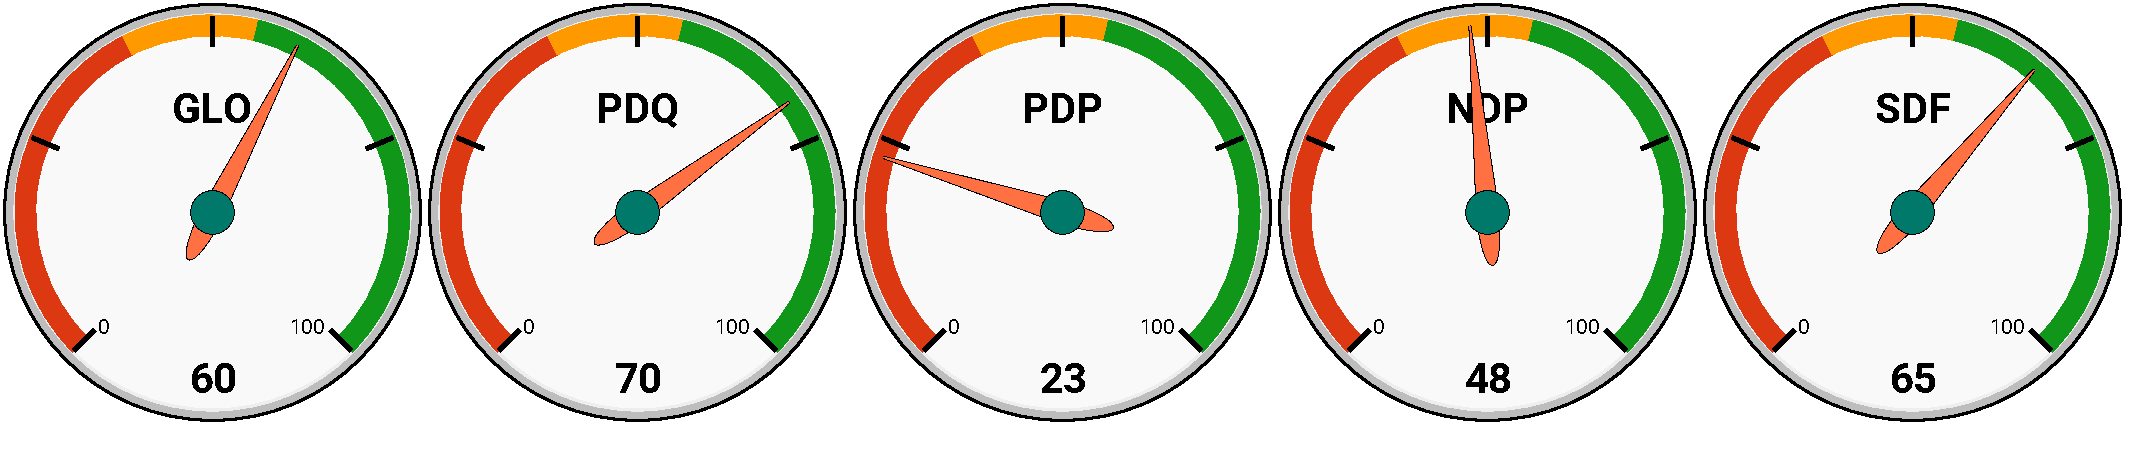
\includegraphics[width=1\linewidth]{sez/App_Esito/graph/AN_Gulp.pdf}
	\caption{Indice di Gulpease nel periodo di Analisi}
\end{figure}

%\textcolor{ForestGreen}{Ottimale}
%\textcolor{YellowOrange}{Accettabile}
%\textcolor{BrickRed}{Non accettabile}